\documentclass[10pt,twocolumn,a4paper]{article}
% Stand-in layout. Port the content to the official IEEE Access template (ieeeaccess.cls) before submission.
\usepackage[margin=0.75in,columnsep=0.25in]{geometry}
\usepackage[utf8]{inputenc}
\usepackage[T1]{fontenc}
\usepackage{mathptmx}
\usepackage{amsmath,amssymb,amsfonts}
\usepackage{graphicx}
\usepackage{booktabs}
\usepackage{cite}
\usepackage[hyphens]{url}
\usepackage{enumitem}
\setlist{nosep,leftmargin=1.4em}
\usepackage{tikz}
\usetikzlibrary{arrows.meta,positioning,calc}
\usepackage[ruled,vlined,linesnumbered,noend]{algorithm2e}
\usepackage[labelfont=bf,font=small]{caption}
\usepackage{microtype}
\setlength{\parskip}{0pt}
\renewcommand{\arraystretch}{1.08}
\newcommand{\E}{\mathbb{E}}
\newcommand{\CN}{\mathcal{CN}}
\newcommand{\tr}{\operatorname{tr}}
\newcommand{\diag}{\operatorname{diag}}

\title{\bfseries Rank-Limited Multiuser Multiplexing in Lens-Antenna Beamspace Systems Aided by an Active RIS: A Practical Energy-Efficiency Study}
\author{\itshape [Author names and affiliations to be completed]}
\date{}

\begin{document}
\maketitle

\begin{abstract}
Active reconfigurable intelligent surfaces (RISs) amplify the reflected signal and can restore a usable link when the direct path is blocked, but their combination with a lens-antenna (beamspace) base station, where RF chains dominate hardware cost, has not been evaluated with a saturating amplifier model and a common power account. This paper reports a simulation-based practical study of a 28~GHz downlink in which a base station with a 64-beam lens array and $N_s$ selected beams serves $K\le 16$ single-antenna users through a 128-element active RIS with Rapp-type amplifiers. We (i) analyse the amplifier with a Bussgang decomposition, which agrees with symbol-level simulation within 0.15~bit/s/Hz on average (0.46\%); (ii) show that the number of users that can be served simultaneously is limited by the effective rank of the BS--RIS channel, so that serving users in time-shared groups raises the average sum-rate for $K=16$ from 30.7 to 39.8~bit/s/Hz in a 16-path channel; (iii) quantify energy efficiency (EE) under an explicit power model, where operating with the best number of RF chains per channel draw gives on average 2.44$\times$ (range 1.55--3.75$\times$) the EE of a 64-RF-chain design that uses the same RIS design procedure, and 1.65--2.75$\times$ under literature-based variations of the RF-chain and RIS-element power; and (iv) find that selecting beams with a linear-amplifier model instead of the saturation model costs little in the cases tested. All designs are heuristic (regularised ZF, gradient phase refinement, greedy beam selection); results cover $K\le16$, one geometry and 30 channel draws per setting, and several power constants are assumptions. The study therefore indicates operating regimes rather than optimality bounds. Code and raw results are public.
\end{abstract}

\begin{center}\small\textbf{Index Terms:} active RIS, beamspace MIMO, lens antenna array, energy efficiency, amplifier saturation, user grouping, millimeter wave.\end{center}

\section{Introduction}
Millimeter-wave links are easily blocked, and reconfigurable intelligent surfaces (RISs) are a low-cost way to create alternative paths. A passive RIS, however, suffers from double path loss: the reflected link attenuates by the product of the BS--RIS and RIS--user losses, so its gain is limited when the direct path is available and the budget is tight. Active RISs mitigate this by amplifying the reflected signal with reflection-type amplifiers at the cost of extra DC power and amplified noise \cite{long2021,zhang2023}.

On the base-station (BS) side, lens-antenna arrays convert the antenna domain into a sparse beamspace so that only a few beams, each with its own RF chain, need to be active \cite{zeng2016,sayeed2013,wang2017,shen2019}. The combination of lens-based beamspace MIMO with RISs has been studied for passive or phase-only surfaces \cite{wanggc2020,liu2021,pal2023,abdullah2025}, and RISs have been proposed as a way to reduce the number of RF chains needed to approach massive-MIMO performance \cite{interdonato2024}.

\textbf{Gap and position.} In the literature we examined (a non-exhaustive web search, November 2026), we did not find a study that jointly considers (a) an active RIS with a saturating amplifier model, (b) beam selection at a lens-antenna BS with a limited number of RF chains, and (c) an energy-efficiency metric that charges both RF chains and per-element RIS amplifier power. This paper therefore does \emph{not} claim a new optimisation algorithm; it is a practical evaluation study whose value lies in identifying which design variables matter under these coupled constraints, with all assumptions stated and all code and data released.

\textbf{Contributions.}
\begin{enumerate}
\item A Bussgang-based analytical model of the Rapp-amplifier active RIS inside a beamspace downlink, validated against symbol-level simulation (Section~\ref{sec:val}).
\item A quantification of the rank limit: because the BS--RIS channel has few resolvable paths and the direct link is blocked, only a few users can be multiplexed at once; time-sharing user groups of size close to the effective rank gives higher average sum-rate and EE than serving all users together (Section~\ref{sec:rank}).
\item An EE study that charges RF chains, the BS amplifier, the RIS amplifier output and the per-element RIS DC power, with a sensitivity analysis over literature-based ranges of the RF-chain and element power (Section~\ref{sec:ee}).
\item A negative/neutral finding: in the tested scenarios, ranking beam sets with a linear amplifier model gives nearly the same ordering as with the saturation model (Section~\ref{sec:dec}).
\end{enumerate}
Section~\ref{sec:rel} summarises related work, Section~\ref{sec:sys} gives the system model, Section~\ref{sec:des} the design procedure, Section~\ref{sec:setup} the simulation setup, Section~\ref{sec:res} the results, and Section~\ref{sec:lim} the limitations.

\section{Related Work}\label{sec:rel}
\textbf{Active RIS.} Long \emph{et al.} introduced the active RIS with negative-resistance loads and studied a SIMO system, balancing signal gain against amplified RIS-correlated noise \cite{long2021}. Zhang \emph{et al.} proposed a signal model for an active RIS verified with a fabricated element, analysed the asymptotic gain and designed joint transmit/reflect beamforming for multi-user MISO sum-rate maximisation \cite{zhang2023}. Hybrid active--passive RIS transmitters have been designed for EE \cite{huang2024}. Further work addresses practical beamforming, hardware impairments and circuit-level modelling of active RISs \cite{yang2024,peng2024,gavriilidis2025}.

\textbf{Lens-antenna and beamspace MIMO.} Lens arrays exploit angle-dependent energy focusing and the angular sparsity of mmWave channels to reduce the number of RF chains \cite{zeng2016,sayeed2013}. Beamspace MIMO-NOMA for spectrum and energy efficiency was studied in \cite{wang2017}, beamspace precoding with beam selection in \cite{shen2019}, and max-min fairness for beamspace MIMO-NOMA in \cite{jiao2022}.

\textbf{RIS with beamspace/lens BS.} Table~\ref{tab:rel} lists the closest works we identified. The first four consider RIS-aided lens or beamspace systems with phase-only surfaces; none, to our knowledge, models amplifier saturation.

\begin{table}[t]\centering\caption{Closest related studies (as described in their abstracts/titles; ``phase-only'' = surface with phase control only).}\label{tab:rel}\small
\begin{tabular}{@{}p{1.55cm}p{1.9cm}p{1.9cm}p{2.1cm}@{}}\toprule
Work & RIS & BS side & Focus\\\midrule
\cite{wanggc2020} & phase-only, multiple IRSs & lens array & EE, AO\\
\cite{liu2021} & phase-only IRS & lens, NOMA & weighted sum-rate\\
\cite{pal2023} & distributed RIS & beamspace & beam selection, max-min\\
\cite{abdullah2025} & multi-RIS & beamspace & PSO, sum-rate\\
\cite{interdonato2024} & active and passive & small array + RIS & SE, max-min\\
\cite{zhang2023} & active, verified model & multi-antenna BS & sum-rate\\
This paper & active, Rapp saturation & lens, beam selection & sum-rate, EE, rank limit\\\bottomrule
\end{tabular}\end{table}

\section{System Model}\label{sec:sys}
\subsection{Scenario and signal model}
A BS with an $M$-antenna lens array transmits to $K$ single-antenna users through an RIS with $N$ elements (Fig.~\ref{fig:sys}). The direct BS--user link is blocked. The lens is modelled as an ideal unitary DFT $\mathbf U\in\mathbb C^{M\times M}$ whose $m$-th column is the beam toward $\sin\varphi_m=(2m-(M-1))/M$. Only the beams in a set $\mathcal S$ with $|\mathcal S|=N_s$ have an RF chain; $\mathbf U_{\mathcal S}$ collects the selected columns. With a beamspace precoder $\mathbf W\in\mathbb C^{N_s\times K}$ and symbols $\mathbf s\sim\CN(\mathbf 0,\mathbf I_K)$ the transmit vector is $\mathbf x=\mathbf U_{\mathcal S}\mathbf W\mathbf s$ with $\|\mathbf W\|_F^2=P_{\rm BS}$.

\begin{figure}[t]\centering
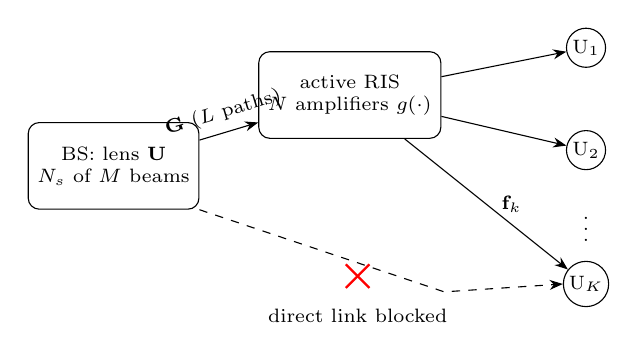
\begin{tikzpicture}[x=1cm,y=1cm,>=Stealth,font=\scriptsize,every node/.style={align=center}]
\node[draw,rounded corners,minimum width=1.6cm,minimum height=1.1cm] (bs) at (0,0) {BS: lens $\mathbf U$\\ $N_s$ of $M$ beams};
\node[draw,rounded corners,minimum width=1.7cm,minimum height=1.1cm] (ris) at (3.0,0.9) {active RIS\\ $N$ amplifiers $g(\cdot)$};
\node[draw,circle,inner sep=1pt] (u1) at (6.0,1.5) {U$_1$};
\node[draw,circle,inner sep=1pt] (u2) at (6.0,0.2) {U$_2$};
\node (u3) at (6.0,-0.7) {$\vdots$};
\node[draw,circle,inner sep=1pt] (uK) at (6.0,-1.5) {U$_K$};
\draw[->] (bs) -- node[above,sloped]{$\mathbf G\ (L$ paths)} (ris);
\draw[->] (ris) -- (u1); \draw[->] (ris) -- (u2); \draw[->] (ris) -- node[right,xshift=2pt]{$\mathbf f_k$} (uK);
\draw[dashed,->] (bs.south east) -- (4.2,-1.6) -- (uK.west);
\node at (3.1,-1.9) {direct link blocked};
\draw[red,thick] (2.95,-1.25) -- (3.25,-1.55); \draw[red,thick] (3.25,-1.25) -- (2.95,-1.55);
\end{tikzpicture}
\caption{System model: lens-antenna BS with beam selection, active RIS with per-element amplifiers, $K$ single-antenna users, blocked direct link.}\label{fig:sys}
\end{figure}

The signal arriving at RIS element $n$ is $u_n=[\mathbf G\mathbf x]_n+v_n$ with $v_n\sim\CN(0,\sigma_v^2)$ the amplifier-input noise. The RIS applies a unit-modulus phase $e^{j\theta_n}$ and amplifies with the memoryless Rapp characteristic \cite{rapp1991} (smoothness factor 2)
\begin{equation}
g(u)=\frac{p\,u}{\bigl(1+(p|u|/A)^{4}\bigr)^{1/4}},\label{eq:rapp}
\end{equation}
where $p$ is the small-signal amplitude gain (taken equal for all elements) and $A$ the output saturation amplitude, set as $A^2=P_{\rm RIS}/N$. The user signal is
\begin{equation}
\mathbf r=\mathbf F\,\diag(e^{j\boldsymbol\theta})\,g(\mathbf u)+\mathbf n,\qquad \mathbf n\sim\CN(\mathbf 0,\sigma^2\mathbf I_K),\label{eq:rx}
\end{equation}
with $\mathbf F\in\mathbb C^{K\times N}$ the RIS--user channel (row $\mathbf f_k$).

\subsection{Channels}
The BS--RIS channel is a sum of $L$ paths,
\begin{equation}
\mathbf G=\sqrt{\mathrm{PL}_G}\sum_{l=1}^{L}c_l\,\mathbf a_N(\psi_l)\mathbf a_M(\phi_l)^H,\label{eq:G}
\end{equation}
where $\mathbf a_X(\omega)=[1,e^{j\pi\omega},\dots,e^{j\pi(X-1)\omega}]^T$ (half-wavelength spacing), $\sin$-domain angles $\phi_l,\psi_l\sim\mathcal U(-0.85,0.85)$, $\sum_l|c_l|^2=1$, path~1 carries 70\% of the power, the remaining 30\% is split by a symmetric Dirichlet draw, and the phases are uniform. Hence $\|\mathbf G\|_F^2\approx\mathrm{PL}_G NM$ (exact up to path cross-terms) with the free-space loss $\mathrm{PL}_G=(\lambda/4\pi d_{BR})^2$ and unit antenna gains. The RIS--user channel is line-of-sight: $\mathbf f_k=\sqrt{\mathrm{PL}_F}\,\gamma_k\,\mathbf a_N(\chi_k)^H$ with random phase $\gamma_k$, free-space loss $\mathrm{PL}_F$ at $d_{RU}$ and well-separated directions $\chi_k$. No shadowing or small-scale fading beyond this structure is modelled. Because $\operatorname{rank}\mathbf G\le L$,
\begin{equation}
\operatorname{rank}\bigl(\mathbf F\diag(\boldsymbol\kappa\odot e^{j\boldsymbol\theta})\mathbf G\mathbf U_{\mathcal S}\bigr)\le\min\{K,L,N_s\},\label{eq:rank}
\end{equation}
which is the origin of the rank limit studied in Section~\ref{sec:rank} (a standard linear-algebra bound, not claimed as new).

\subsection{Bussgang model of the amplifier}
For $u_n\sim\CN(0,P_n)$ with $P_n=\|\mathbf e_n^T\mathbf G\mathbf U_{\mathcal S}\mathbf W\|^2+\sigma_v^2$, Bussgang's theorem \cite{buss1952} gives $g(u_n)=\kappa_n u_n+d_n$, where $\kappa_n=\E[g(u_n)u_n^*]/P_n$ and the distortion $d_n$ is uncorrelated with $u_n$ and has power $\sigma_{d,n}^2=\E|g(u_n)|^2-\kappa_n^2P_n$. For the Rapp function, $\kappa_n$ and $\E|g(u_n)|^2$ are one-dimensional integrals over $t=|u_n|^2/P_n\sim\mathrm{Exp}(1)$ (Appendix); we evaluate them with a 96-point Gauss--Laguerre rule. With the usual approximation that distortion terms are independent across elements, the SINR of user $k$ is
\begin{equation}
\gamma_k=\frac{|T_{kk}|^2}{\sum_{j\ne k}|T_{kj}|^2+\sum_n|f_{kn}|^2\bigl(\kappa_n^2\sigma_v^2+\sigma_{d,n}^2\bigr)+\sigma^2},\label{eq:sinr}
\end{equation}
with $\mathbf T=\mathbf F\diag(\boldsymbol\kappa\odot e^{j\boldsymbol\theta})\mathbf G\mathbf U_{\mathcal S}\mathbf W$. The rate is $R_k=\log_2(1+\gamma_k)$ and the RIS output power is $P_{\rm out}=\sum_n\E|g(u_n)|^2\le P_{\rm RIS}$. The independence approximation and Gaussian input are checked against symbol-level simulation in Section~\ref{sec:val}.

\subsection{Power consumption}
The total consumption is
\begin{equation}
P_{\rm tot}=\frac{P_{\rm BS}}{\eta_{\rm BS}}+N_sP_{\rm RF}+P_{\rm fix}+\frac{P_{\rm out}}{\eta_{\rm RIS}}+N P_{\rm el},\label{eq:power}
\end{equation}
with $P_{\rm el}=P_{\rm el}^{\rm act}$ for the active RIS (amplifier bias per element) and, for the passive reference, $P_{\rm out}$ is omitted and $P_{\rm el}=P_{\rm el}^{\rm pas}$. Energy efficiency is $\mathrm{EE}=\sum_kR_k/P_{\rm tot}$ in bit/s/Hz/W. The constants (Table~\ref{tab:par}) are ranges from the literature or explicit assumptions; Section~\ref{sec:ee} tests their influence.

\section{Design Procedure}\label{sec:des}
\subsection{Problem and approach}
For a given user set and $N_s$ the goal is to maximise $\sum_kR_k$ over $(\mathcal S,\mathbf W,p,\boldsymbol\theta)$ subject to $|\mathcal S|=N_s$, $\|\mathbf W\|_F^2\le P_{\rm BS}$, $P_{\rm out}\le P_{\rm RIS}$ and $|e^{j\theta_n}|=1$. This problem is non-convex and we do not solve it to optimality. The procedure below is a heuristic pipeline; $N_s$ is swept rather than optimised, and EE is evaluated afterwards.

\textbf{Phase gradient.} For fixed $\mathbf W$ and $p$ the powers $P_n$, hence $\kappa_n$ and $\sigma_{d,n}^2$, do not depend on $\boldsymbol\theta$. Writing $c_{kj}[n]=f_{kn}\kappa_n[\mathbf G\mathbf U_{\mathcal S}\mathbf W]_{nj}$, \eqref{eq:sinr} becomes
\begin{equation}
\gamma_k=\frac{|\mathbf c_{kk}^T e^{j\boldsymbol\theta}|^2}{\sum_{j\ne k}|\mathbf c_{kj}^Te^{j\boldsymbol\theta}|^2+\nu_k},
\end{equation}
so the objective and its gradient with respect to $\boldsymbol\theta$ are available in closed form. We ascend the proportional-fair objective $\sum_k\log_2(R_k+\epsilon)$, $\epsilon=0.5$, with Adam \cite{kingma2015}; plain sum-rate maximisation tended to starve weak users in earlier trials.

\begin{algorithm}[t]\caption{Design for one user group (one time slot)}\label{alg:design}\small
\KwIn{channels $\mathbf G,\mathbf F$ of the group, $N_s$, $P_{\rm BS}$, $P_{\rm RIS}$}
Align RIS phases with a ZF precoder over all $M$ beams and rank the beams by cascaded energy\;
\eIf{$N_s\ge 25$}{$\mathcal S\leftarrow$ all $M$ beams (full-digital reference)}{greedy forward selection on the \emph{linear}-amplifier model: start from the $K$ strongest beams; add, from the $\max\{24,2N_s\}$ strongest, the beam that maximises the sum-rate (8-point $p$ grid) until $|\mathcal S|=N_s$}
Initialise $\boldsymbol\theta$ by alternating phase alignment on $\mathcal S$\;
\For{outer round $=1,2$}{
 choose $(p,\alpha)$ on a grid ($p\in[1,100]$, 16 log-spaced points; $\alpha\in\{0,0.1,0.3,1\}$) maximising the sum-rate of the RZF precoder \cite{peel2005} built on the effective channel including $\kappa_n$ (two fixed-point updates), subject to $P_{\rm out}\le P_{\rm RIS}$\;
 refine $\boldsymbol\theta$: 40 Adam steps on the proportional-fair objective with $\mathbf W,p$ fixed\;
 keep the design with the best objective\;}
\KwOut{$\mathcal S,\mathbf W,p,\boldsymbol\theta$}\end{algorithm}

\subsection{User grouping}
When $K$ exceeds what the channel rank supports, users are split into $\lceil K/g\rceil$ groups served in equal time slots, so each user's rate is $R_k/\lceil K/g\rceil$. Groups are built greedily: the strongest remaining user (largest $\|\mathbf f_k\|$) starts a group and users with the smallest maximum normalised correlation $|\mathbf f_i\mathbf f_j^H|/(\|\mathbf f_i\|\|\mathbf f_j\|)$ to current members are added until the group holds $g$ users. Algorithm~\ref{alg:design} runs separately in each slot, and $P_{\rm tot}$ is averaged over slots. We report the sum-rate, the minimum user rate, Jain's index \cite{jain1984} and EE, all time-averaged.

\subsection{Complexity}
The $K\times K\times N$ tensor of $c_{kj}[n]$ is formed once per refinement call and each Adam step then costs $\mathcal O(K^2N)$. One evaluation of \eqref{eq:sinr} costs $\mathcal O(NN_sK)$ plus $N$ one-dimensional quadratures; each greedy step evaluates the grid design for up to $\max\{24,2N_s\}$ candidates, so beam selection dominates for $N_s\le24$. We make no low-complexity claim: the implementation is unoptimised Python and the whole set of configurations for one scene takes a median 6.2~s, 16.9~s and 38.5~s for $K=4,8,16$ on a shared two-core CPU (the maximum was 66.6~s for $K=16$). Full-digital designs avoid the greedy search, so run-time is not comparable between arms.

\section{Simulation Setup}\label{sec:setup}
Table~\ref{tab:par} lists all parameters. For each $(K,L)$ we simulate $n=30$ independent channel draws (seeds $100+d$; $d=0,\dots,n-1$ for every $(K,L)$, so the draw index is shared but channels differ across $K$ and $L$). Plots and tables report means with 95\% confidence half-widths $1.96\,s/\sqrt n$ unless noted. Schemes: (i) \emph{beamspace}: group size $g\in\{4,8,K\}$ and $N_s\in\{\lceil1.5g\rceil,\lceil3g\rceil,\lceil6g\rceil\}$ (any value above 24 is replaced by all 64 beams) plus the full-digital arm $N_s=64$; (ii) a \emph{passive RIS} reference with the same grouping, $p=1$, no amplifier noise and $P_{\rm el}^{\rm pas}$.

\begin{table}[t]\centering\caption{Simulation parameters. ``Set'' = chosen by us; ``Lit.'' = within a range reported in the cited works; ``Assumed'' = our assumption without source.}\label{tab:par}\footnotesize
\begin{tabular}{@{}p{3.05cm}p{3.15cm}p{0.85cm}@{}}\toprule
Parameter & Value & Source\\\midrule
Carrier frequency $f_c$ & 28 GHz & Set\\
Lens beams $M$ / RF chains $N_s$ & 64 / $\{6,12,24,64\}$ & Set\\
RIS elements $N$ & 128 (ULA, $\lambda/2$) & Set\\
Users $K$, group size $g$ & $\{4,8,16\}$, $\{4,8,K\}$ & Set\\
BS--RIS / RIS--user distance & 20 m / 10 m, free space & Set\\
BS--RIS paths $L$ & 6, 16 (70\% main path) & Set\\
$P_{\rm BS}$, $P_{\rm RIS}$ & 1 W (30 dBm), 0.1 W (20 dBm) & Set\\
Saturation amplitude $A$ & $\sqrt{P_{\rm RIS}/N}$ (0 dB back-off) & Set\\
$\sigma_v^2=\sigma^2$ & $2\times10^{-12}$ W ($-87$ dBm) & Set\\
RZF load $\alpha$; PF const.\ $\epsilon$ & $\{0,.1,.3,1\}$; 0.5 & Set\\
$P_{\rm RF}$ per chain & 250 mW (100--250) \cite{koc,qi2022,hao2017} & Lit.\\
$P_{\rm el}^{\rm act}$ per element & 20 mW (8--26.5) \cite{gavriilidis2025} & Lit.\\
$P_{\rm el}^{\rm pas}$ per element & 1 mW & Assumed\\
$\eta_{\rm BS}$, $\eta_{\rm RIS}$ & 0.4, 0.4 & Assumed\\
$P_{\rm fix}$ & 1 W & Assumed\\
Draws per $(K,L)$ & 30 & Set\\\bottomrule
\end{tabular}\end{table}

\section{Results}\label{sec:res}
\subsection{Validation of the Bussgang model}\label{sec:val}
For 30 designs ($(K,L,N_s)\in\{(4,6,12),(8,16,12),(16,16,24)\}$, ten draws each) we compared the analytical sum-rate with a symbol-level simulation that passes Gaussian symbols through \eqref{eq:rapp} (60\,000 symbols per design, SINR from the empirical correlation with the transmitted symbols). The mean absolute difference was 0.15~bit/s/Hz (0.46\% relative), the maximum 1.30~bit/s/Hz (4.0\%), and the analytical rate was on average 0.13~bit/s/Hz \emph{higher}. Reported analytical rates are therefore slightly optimistic. The comparison does not cover non-Gaussian (finite-alphabet) inputs.

\subsection{Rank limit and user grouping}\label{sec:rank}
Fig.~\ref{fig:svd} shows the singular values of $\mathbf G$ for draws 0--19 (the first 20 seeds of the grid). With a $-20$~dB threshold, the median effective rank is 5.5 for $L=6$ and 10 for $L=16$, i.e.\ well below $K=16$, consistent with \eqref{eq:rank}.

\begin{figure}[t]\centering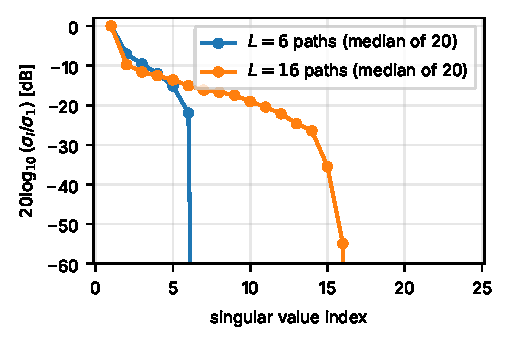
\includegraphics[width=0.95\columnwidth]{figs/fig_svd.pdf}\caption{Singular values of $\mathbf G$ (median of 20 draws, $-20$~dB rank threshold used in the text).}\label{fig:svd}\end{figure}

Fig.~\ref{fig:group} and Table~\ref{tab:main} show the effect on $K=16$ users. For $L=16$, the best group size among $\{4,8,16\}$ is $g=8$: with $N_s=1.5g$ the sum-rate is 39.8~bit/s/Hz versus 30.7 for serving all users together, and the minimum user rate rises from 0.85 to 2.34~bit/s/Hz. Taking the best $N_s$ for each group size, the best sum-rates are 32.0, 43.8 and 30.7~bit/s/Hz for $g=4,8,16$. For $L=6$ the best group size is $g=4$, with 29.9, 22.2 and 13.2~bit/s/Hz for $g=4,8,16$ (best $N_s$ each). In this channel the best $g$ is just below the effective rank; only three values of $g$ were tested, so we do not claim a closed-form rule.

For $L=6$, however, fairness remains poor even with the proportional-fair phase objective: at $g=4$ the average minimum user rate is only 0.46~bit/s/Hz and Jain's index 0.81. Part of the sum-rate benefit therefore comes from favouring users with strong channels, and the grouping rule uses only RIS-side correlations and norms (no rate feedback).

\begin{figure*}[t]\centering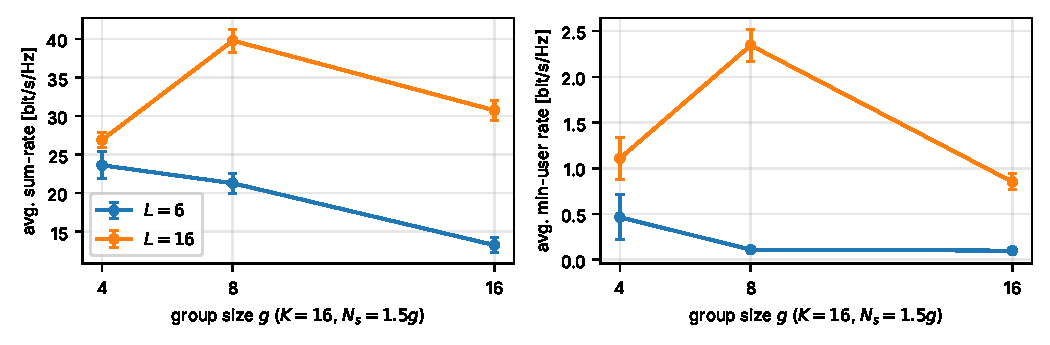
\includegraphics[width=0.78\textwidth]{figs/fig_group.pdf}\caption{Effect of group size $g$ at $K=16$ with $N_s=1.5g$: average sum-rate (left) and minimum user rate (right), with 95\% CI over the channel draws.}\label{fig:group}\end{figure*}

\begin{table*}[t]\centering\caption{$K=16$: selected configurations (mean over $n=30$ draws; $\pm$ = 95\% CI). Rates are time-averaged over slots; ``passive'' uses $N_s=12$, $g=4$.}\label{tab:main}\small
\begin{tabular}{@{}rlccccc@{}}\toprule
$L$ & Configuration & Sum-rate [bit/s/Hz] & Min-user rate & Jain & $P_{\rm tot}$ [W] & EE [bit/s/Hz/W]\\\midrule
6 & $g{=}4,N_s{=}6$ & 23.6$\pm$1.8 & 0.46 & 0.81 & 7.6 & 3.11$\pm$0.23 \\
6 & $g{=}4,N_s{=}12$ & 28.2$\pm$1.1 & 1.03 & 0.93 & 9.1 & 3.11$\pm$0.12 \\
6 & $g{=}4,N_s{=}64$ & 29.9$\pm$0.7 & 1.64 & 0.99 & 22.1 & 1.35$\pm$0.03 \\
6 & $g{=}8,N_s{=}12$ & 21.3$\pm$1.3 & 0.11 & 0.69 & 9.1 & 2.34$\pm$0.14 \\
6 & $g{=}8,N_s{=}64$ & 19.1$\pm$1.0 & 0.21 & 0.74 & 22.1 & 0.87$\pm$0.05 \\
6 & $g{=}16,N_s{=}24$ & 13.2$\pm$1.0 & 0.10 & 0.52 & 12.1 & 1.10$\pm$0.08 \\
6 & $g{=}16,N_s{=}64$ & 11.9$\pm$0.5 & 0.12 & 0.60 & 22.1 & 0.54$\pm$0.02 \\
6 & passive RIS, $g{=}4,N_s{=}12$ & 0.8$\pm$0.1 & 0.00 & 0.34 & 6.6 & 0.13$\pm$0.02 \\
\midrule
16 & $g{=}4,N_s{=}6$ & 26.9$\pm$1.0 & 1.11 & 0.95 & 7.6 & 3.55$\pm$0.13 \\
16 & $g{=}4,N_s{=}12$ & 31.2$\pm$0.5 & 1.75 & 0.99 & 9.1 & 3.43$\pm$0.05 \\
16 & $g{=}4,N_s{=}64$ & 31.8$\pm$0.4 & 1.89 & 1.00 & 22.1 & 1.44$\pm$0.02 \\
16 & $g{=}8,N_s{=}12$ & 39.8$\pm$1.5 & 2.34 & 0.99 & 9.1 & 4.39$\pm$0.16 \\
16 & $g{=}8,N_s{=}64$ & 43.8$\pm$0.9 & 2.69 & 1.00 & 22.1 & 1.99$\pm$0.04 \\
16 & $g{=}16,N_s{=}24$ & 30.7$\pm$1.3 & 0.85 & 0.90 & 12.1 & 2.55$\pm$0.11 \\
16 & $g{=}16,N_s{=}64$ & 29.5$\pm$1.1 & 1.05 & 0.93 & 22.1 & 1.34$\pm$0.05 \\
16 & passive RIS, $g{=}4,N_s{=}12$ & 0.6$\pm$0.1 & 0.00 & 0.43 & 6.6 & 0.08$\pm$0.01
\\
\bottomrule
\end{tabular}\end{table*}

\subsection{Energy efficiency versus number of RF chains}\label{sec:ee}
Fig.~\ref{fig:ee} plots EE and sum-rate for $g=4$ against $N_s$. EE peaks at few RF chains: the best EE among the tested active-RIS configurations at $K=16$ is 4.39~bit/s/Hz/W for $L=16$ ($g=8$, $N_s=12$) and 3.11 for $L=6$ ($g=4$, $N_s=6$), whereas $g=4$ with all 64 beams reaches only 1.44 ($L=16$) and 1.35 ($L=6$) because the total power rises from 9.1 to 22.1~W. Going from $N_s=12$ to 64 at $g=4$ raises the sum-rate by only 2.1\% ($L=16$) and 6.0\% ($L=6$), so the additional chains mostly add power.

\begin{figure*}[t]\centering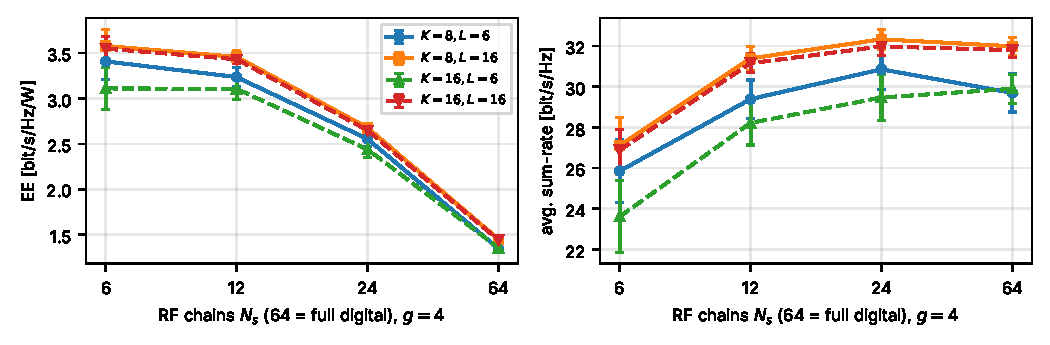
\includegraphics[width=0.78\textwidth]{figs/fig_ee.pdf}\caption{EE (left) and sum-rate (right) versus the number of RF chains for $g=4$ ($N_s=64$ is full-digital). Mean with 95\% CI.}\label{fig:ee}\end{figure*}

Table~\ref{tab:ratio} gives the paired EE ratio between the best beamspace configuration and the full-digital configuration with the same group size, over all draws and group sizes in $\{4,8,K\}$ ($360$ pairs): mean 2.44$\times$, minimum 1.55$\times$, maximum 3.75$\times$. Because the best $N_s$ is chosen per draw, this ratio is an optimistic ``oracle'' figure; for fixed configurations the paired ratios (no per-draw selection, vs.\ $N_s=64$ at the same $g$) are 2.44$\times$ ($g=4$, $N_s=6$), 2.38$\times$ ($g=4$, $N_s=12$, minimum 1.26) and 2.51$\times$ ($g=8$, $N_s=12$, minimum 1.80). The mean sum-rate loss of the best-EE beamspace configuration relative to full-digital is 0.9\% (maximum 37.7\% in a single draw). That a 64-beam design is on average barely better than a few-beam subset suggests that our heuristic does not exploit the extra beams (in the ideal case a full-digital design can never be worse than a beam subset). The EE ratios are therefore partly a property of our design procedure and should not be read as guaranteed hardware gains.

\begin{table}[t]\centering\caption{Paired EE ratio, best beamspace / full-digital (95\% CI).}\label{tab:ratio}\small
\begin{tabular}{@{}rcc@{}}\toprule $K$ & $L$ & ratio\\\midrule4 & 6 & 2.60$\pm$0.12 \\
4 & 16 & 2.57$\pm$0.09 \\
8 & 6 & 2.76$\pm$0.10 \\
8 & 16 & 2.40$\pm$0.06 \\
16 & 6 & 2.40$\pm$0.09 \\
16 & 16 & 2.21$\pm$0.06
\\
\bottomrule\end{tabular}\end{table}

\textbf{Sensitivity to power constants.} Table~\ref{tab:sens} recomputes the best-per-draw EE ratio with $P_{\rm RF}\in\{100,160,250\}$~mW and $P_{\rm el}^{\rm act}\in\{8.5,20,26.5\}$~mW, i.e.\ literature-based ranges. The mean ratio stays between 1.65 and 2.75, and the minimum over draws is 1.18 in the worst case. Constants outside these ranges, or different $\eta_{\rm BS}$, $\eta_{\rm RIS}$, $P_{\rm fix}$, were not varied; the largest benefit occurs when RF chains are expensive relative to the RIS elements.

\begin{table}[t]\centering\caption{Sensitivity of the best-per-draw EE ratio to $P_{\rm RF}$ and $P_{\rm el}^{\rm act}$ (all $(K,L,g)$ combined).}\label{tab:sens}\small
\begin{tabular}{@{}rrcc@{}}\toprule $P_{\rm RF}$ [mW] & $P_{\rm el}$ [mW] & mean ratio & min ratio\\\midrule100 & 8.5 & 1.89 & 1.31 \\
100 & 20.0 & 1.72 & 1.21 \\
100 & 26.5 & 1.65 & 1.18 \\
160 & 8.5 & 2.28 & 1.49 \\
160 & 20.0 & 2.04 & 1.39 \\
160 & 26.5 & 1.94 & 1.35 \\
250 & 8.5 & 2.75 & 1.65 \\
250 & 20.0 & 2.44 & 1.55 \\
250 & 26.5 & 2.32 & 1.50
\\
\bottomrule\end{tabular}\end{table}

\subsection{Passive RIS reference}
With the same BS power and a passive RIS ($p=1$) the average sum-rate at $K=8$, $L=16$, $g=4$, $N_s=12$ is 0.6~bit/s/Hz versus 31.4 for the active RIS; across all $(K,L)$ draws it never exceeds 2.1~bit/s/Hz (Table~\ref{tab:main} gives the $K=16$ case). This large gap reflects the chosen link budget (blocked direct link, 1~W BS, $30$ m total reflected path) and the fact that the active RIS adds up to 0.1~W of output power; the EE column accounts for the extra consumption, but we did not evaluate the passive RIS with a larger BS power or more RIS elements. The comparison is scenario-specific.

\subsection{Saturation and beam selection}\label{sec:dec}
Because the beam selection used in Section~\ref{sec:rank}--\ref{sec:ee} ranks beams with a linear amplifier, we tested whether this ordering matters. For 4 channel draws ($K=4$, $L=6$, $P_{\rm RIS}=10$~dBm in this diagnostic), saturation back-offs $\beta=10\log_{10}(A^2N/P_{\rm RIS})\in\{-5,0,5\}$~dB and 120 random sets of six beams among the 20 strongest, we compared the sum-rate ordering under a linear amplifier and under the saturating amplifier. The Spearman correlation was lowest, 0.951, at $\beta=-5$~dB and at least 0.998 at $\beta=+5$~dB; the best beam set under the linear model coincided with the best one under saturation in 10 of 12 cases, and the largest rate loss from using the linear-model choice was 1.17~bit/s/Hz. Saturation therefore has a modest influence on which beams to select when RIS input power is spread by about 2.6--6.0~dB across elements. This test used random beam sets and $K=4$ only; it does not exclude a larger interaction for other geometries or stronger compression.

\section{Discussion and Limitations}\label{sec:lim}
\textbf{What the results support.} (i) Under a blocked direct link and a few resolvable BS--RIS paths, the number of simultaneously served users is bounded by the effective channel rank, and time-shared groups of comparable size raise the average sum-rate and EE. (ii) In our power model, EE is maximised with 6--12 RF chains rather than 64. (iii) The ordering of beams is only weakly sensitive to amplifier saturation in the tested cases.

\textbf{What they do not support.} No claim is made about optimality, about superiority over joint-optimisation algorithms (none was implemented as a baseline), or about scaling beyond $K=16$ ($K=32$ was dropped for computing cost). Results are for one geometry (20~m/10~m, free space), idealised channel and lens models (no blockage on the RIS--user side, no beam-squint, no lens loss), perfect CSI, and uniform amplifier gain across RIS elements. The designs are heuristics; sum-rate is not monotonic in $N_s$ in our results, which shows the pipeline leaves performance unrealised. Several power constants ($\eta_{\rm BS}$, $\eta_{\rm RIS}$, $P_{\rm fix}$, $P_{\rm el}^{\rm pas}$) are assumptions; the best $N_s$ per draw is an oracle choice. Rates are analytical (slightly optimistic, Section~\ref{sec:val}), channel draws are 30 per setting, and time-sharing assumes ideal slot allocation with no signalling or switching overhead.

\section{Conclusion}
For a lens-antenna BS serving many users through an active RIS with a blocked direct link, the achievable multiplexing is governed by the effective rank of the BS--RIS channel rather than by the number of users or RF chains. In our simulations, grouping users close to that rank and using a few RF chains gave the best sum-rate/EE trade-off, with EE gains over a 64-RF-chain design of about 2.38$\times$ for fixed $g=4$, $N_s=12$ and between 1.65 and 2.75$\times$ over the tested power constants (best-per-draw). These figures depend on our heuristic design, assumed constants and a single geometry, so they indicate regimes rather than guarantees. Natural next steps are joint optimisation of beams, precoder, phases and non-uniform amplifier gains under the saturation model, $K$ beyond 16, imperfect CSI, and measured lens/amplifier characteristics.

\section*{Data and Code Availability}
Scripts, raw per-draw results (\texttt{results\_S2.jsonl}) and the generator for all tables and figures are in the public repository \url{https://github.com/ApiEdu/How-Much-Gain-Is-Usable-Sum-Rate-Limits-of-Active-RIS-Aided-MU-MISO-Systems} (branch \texttt{beamspace-saturation}; to be merged/tagged at submission).

\appendix
\section{Rapp-amplifier Bussgang moments}
Let $t=|u|^2/P\sim\mathrm{Exp}(1)$ and $\rho=p^2P/A^2$. Then
\begin{align}
\kappa&=p\,\E_t\!\bigl[t\,(1+\rho^2t^2)^{-1/4}\bigr],\\
\E|g(u)|^2&=p^2P\,\E_t\!\bigl[t\,(1+\rho^2t^2)^{-1/2}\bigr],\\
\sigma_d^2&=\E|g(u)|^2-\kappa^2P.
\end{align}
These follow from \eqref{eq:rapp} with $|u|^2=Pt$.

\bibliographystyle{unsrt}
\begin{thebibliography}{99}
\bibitem{long2021} R. Long, Y.-C. Liang, Y. Pei, and E. G. Larsson, ``Active reconfigurable intelligent surface-aided wireless communications,'' \emph{IEEE Trans. Wireless Commun.}, vol. 20, no. 8, pp. 4962--4975, Aug. 2021.
\bibitem{zhang2023} Z. Zhang, L. Dai, X. Chen, C. Liu, F. Yang, R. Schober, and H. V. Poor, ``Active RIS vs. passive RIS: Which will prevail in 6G?'' \emph{IEEE Trans. Commun.}, vol. 71, no. 3, pp. 1707--1725, Mar. 2023.
\bibitem{zeng2016} Y. Zeng and R. Zhang, ``Millimeter wave MIMO with lens antenna array: A new path division multiplexing paradigm,'' \emph{IEEE Trans. Commun.}, vol. 64, no. 4, pp. 1557--1571, Apr. 2016.
\bibitem{sayeed2013} A. Sayeed and J. Brady, ``Beamspace MIMO for high-dimensional multiuser communication at millimeter-wave frequencies,'' in \emph{Proc. IEEE GLOBECOM}, Atlanta, GA, USA, Dec. 2013, pp. 3679--3684.
\bibitem{wang2017} B. Wang, L. Dai, Z. Wang, N. Ge, and S. Zhou, ``Spectrum and energy efficient beamspace MIMO-NOMA for millimeter-wave communications using lens antenna array,'' \emph{IEEE J. Sel. Areas Commun.}, vol. 35, no. 10, pp. 2370--2382, Oct. 2017.
\bibitem{shen2019} W. Shen, X. Bu, X. Gao, C. Xing, and L. Hanzo, ``Beamspace precoding and beam selection for wideband millimeter-wave MIMO relying on lens antenna arrays,'' \emph{IEEE Trans. Signal Process.}, vol. 67, no. 24, pp. 6301--6313, Dec. 2019.
\bibitem{wanggc2020} Y. Wang, H. Lu, D. Zhao, and H. Sun, ``Energy efficiency optimization in IRS-enhanced mmWave systems with lens antenna array,'' in \emph{Proc. IEEE GLOBECOM}, 2020, doi: 10.1109/GLOBECOM42002.2020.9348266.
\bibitem{liu2021} P. Liu, Y. Li, W. Cheng, X. Gao, and X. Huang, ``Intelligent reflecting surface aided NOMA for millimeter-wave massive MIMO with lens antenna array,'' \emph{IEEE Trans. Veh. Technol.}, 2021, doi: 10.1109/TVT.2021.3067938.
\bibitem{pal2023} R. Pal and K. P. Sarawadekar, ``Distributed RIS-assisted mmWave multi-user MIMO beamspace system,'' \emph{AEU -- Int. J. Electron. Commun.}, 2023, doi: 10.1016/j.aeue.2023.154560.
\bibitem{abdullah2025} Z. Abdullah, M. R. Camana, A. B. M. Adam, C. K. Sheemar, E. Lagunas, and S. Chatzinotas, ``Swarm intelligence optimization of multi-RIS aided mmWave beamspace MIMO,'' in \emph{Proc. IEEE VTC2025-Spring}, 2025, doi: 10.1109/VTC2025-Spring65109.2025.11174900.
\bibitem{interdonato2024} G. Interdonato, F. Di Murro, C. D'Andrea, G. Di Gennaro, and S. Buzzi, ``Approaching massive MIMO performance with reconfigurable intelligent surfaces: We do not need many antennas,'' arXiv:2203.07493 (v2), Oct. 2024.
\bibitem{huang2024} A. Huang, X. Mu, L. Guo, and G. Zhu, ``Hybrid active-passive RIS transmitter enabled energy-efficient multi-user communications,'' \emph{IEEE Trans. Wireless Commun.}, vol. 23, no. 9, pp. 10653--10666, Sep. 2024.
\bibitem{yang2024} Y. Yang, Z. Lu, M. Li, R. Liu, and Q. Liu, ``A practical beamforming design for active RIS-assisted MU-MISO systems,'' arXiv:2401.03873, 2024.
\bibitem{peng2024} Z. Peng, Z. Zhang, C. Pan, M. Di Renzo, O. A. Dobre, and J. Wang, ``Beamforming optimization for active RIS-aided multiuser communications with hardware impairments,'' arXiv:2402.10687, 2024.
\bibitem{gavriilidis2025} P. Gavriilidis, D. Mishra, B. Smida, E. Basar, C. Yuen, and G. C. Alexandropoulos, ``Active reconfigurable intelligent surfaces: Circuit modeling and reflection amplification optimization,'' arXiv:2503.24093, 2025.
\bibitem{jiao2022} R. Jiao, L. Dai, W. Wang, F. Lyu, N. Cheng, and X. Shen, ``Max-min fairness for beamspace MIMO-NOMA: From single-beam to multi-beam,'' \emph{IEEE Trans. Wireless Commun.}, vol. 21, no. 2, pp. 739--752, Feb. 2022.
\bibitem{rapp1991} C. Rapp, ``Effects of HPA-nonlinearity on a 4-DPSK/OFDM signal for a digital sound broadcasting system,'' in \emph{Proc. 2nd Eur. Conf. Satell. Commun.}, Li\`ege, Belgium, Oct. 1991, pp. 179--184.
\bibitem{buss1952} J. J. Bussgang, ``Crosscorrelation functions of amplitude-distorted Gaussian signals,'' MIT Res. Lab. Electron., Cambridge, MA, USA, Tech. Rep. 216, Mar. 1952.
\bibitem{kingma2015} D. P. Kingma and J. Ba, ``Adam: A method for stochastic optimization,'' in \emph{Proc. Int. Conf. Learn. Represent. (ICLR)}, 2015, arXiv:1412.6980.
\bibitem{peel2005} C. B. Peel, B. M. Hochwald, and A. L. Swindlehurst, ``A vector-perturbation technique for near-capacity multiantenna multiuser communication---Part I: Channel inversion and regularization,'' \emph{IEEE Trans. Commun.}, vol. 53, no. 1, pp. 195--202, Jan. 2005.
\bibitem{jain1984} R. Jain, D.-M. Chiu, and W. Hawe, ``A quantitative measure of fairness and discrimination for resource allocation in shared computer systems,'' Digital Equipment Corp., Tech. Rep. DEC-TR-301, Sep. 1984.
\bibitem{koc} A. Koc and T. Le-Ngoc, ``Full-duplex mmWave massive MIMO systems: A joint hybrid precoding/combining and self-interference cancellation design,'' arXiv:2104.00191.
\bibitem{qi2022} C. Qi, Q. Liu, X. Yu, and G. Y. Li, ``Hybrid precoding for mixture use of phase shifters and switches in mmWave massive MIMO,'' arXiv:2208.00714.
\bibitem{hao2017} W. Hao, M. Zeng, Z. Chu, and S. Yang, ``Energy-efficient power allocation in millimeter wave massive MIMO with non-orthogonal multiple access,'' arXiv:1707.04520, 2017.
\end{thebibliography}
\end{document}
